%; whizzy document
% latex beamer presentation.
% requires latex and latex-beamer 


%     Tokyo Debian Meeting resources
%     Copyright (C) 2006 Junichi Uekawa

%     This program is free software; you can redistribute it and/or modify
%     it under the terms of the GNU General Public License as published by
%     the Free Software Foundation; either version 2 of the License, or
%     (at your option) any later version.

%     This program is distributed in the hope that it will be useful,
%     but WITHOUT ANY WARRANTY; without even the implied warranty of
%     MERCHANTABILITY or FITNESS FOR A PARTICULAR PURPOSE.  See the
%     GNU General Public License for more details.

%     You should have received a copy of the GNU General Public License
%     along with this program; if not, write to the Free Software
%     Foundation, Inc., 51 Franklin St, Fifth Floor, Boston, MA  02110-1301 USA


\documentclass[dvipdfm]{beamer}
\usetheme{Warsaw}
%  preview (shell-command (concat "xpdf " (replace-regexp-in-string "tex$" "pdf"(buffer-file-name)) "&"))
%  presentation (shell-command (concat "xpdf -fullscreen " (replace-regexp-in-string "tex$" "pdf"(buffer-file-name)) "&"))

\title[Tokyo-Area Debian Meeting]{The Beginning: Debian Multimedia Project}
\subtitle{18 Feb 2006: Tokyo-Area Debian Meeting}
\author{Junichi Uekawa}
\date{18 Feb 2006}

\begin{document}

\frame{\titlepage{}}
 
 \section{Debian Multimedia}
 \subsection{In the Beginning}
 \begin{frame}
  \frametitle{Meaning of DAW}
   DAW: Digital Audio Workstation

  A workstation used in audio recording and editing. Usually consists of
  unusually large amount of memory (max them out!), quiet, high-speed
  disk storage, and inordinate amount of audio I/O. Systems capable of
  10 to 24 track audio input/output is not unusual, and is one of the
  ways music-lovers can waste their money quite efficiently.

 \end{frame}
 
 \begin{frame}
  \frametitle{Meaning of DAW}
  DAW: Debian Audio Workstation

  An adventurous attempt to use Debian to perform recording and mastering
  with many audio tracks. It was known to be a difficult path until
  beginning of 2006. With improvement of real-time response times, it
  became popular by year 2007... (hope)

 \end{frame}


\begin{frame}
\frametitle{State of the Union}
 \begin{itemize}
  \item AGNULA/DeMuDi:
	A project that ran in Europe with some funding for the last few
	years.
	A Custom Debian Distribution focused on Multimedia.
  \item linux-audio-dev: 
	Mailing list for developing audio applications on linux. 
	A very active list where applicaitons like ladspa and jack were born.
	There are frequent postings of new application annoucements also.
  \item Debian-multimedia: A mailing list for multimedia in Debian.
	Required for coordination for things as ladspa and jack.  There
	was a Debian Multimedia-meeting in Brasil in 2004, but the list
	hasn't been very active for the last few years.
 \end{itemize}
\end{frame}

\begin{frame}
\frametitle{Fundamentals}
 \begin{itemize}
  \item audio I/O
  \item MIDI
  \item software effects
  \item software synthesizers
  \item Audio/midi sequencers
 \end{itemize}
\end{frame}

\begin{frame}
\frametitle{Fundamentals, in Linux}
 \begin{itemize}
  \item Audio I/O: ALSA audio, jack
  \item MIDI: ALSA MIDI
  \item Software effects: LADSPA
  \item Software synthesisers: ALSA MIDI-driven, output with jack
  \item audio/MIDI sequencer: audacity, muse, ardour, rosegarden etc.
 \end{itemize}
 Operation is done through Jack audio, and MIDI  (ALSA-midi).
\end{frame}

 \subsection{Available applications}
\begin{frame}
 \frametitle{Using PC keyboard as musical keyboard}
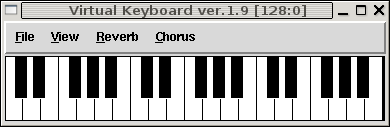
\includegraphics[width=10cm]{image200602/vkeybd.png}\\
 vkeybd, useful for testing out.
\end{frame}

\begin{frame}
 \frametitle{qjackctl: managing connections}
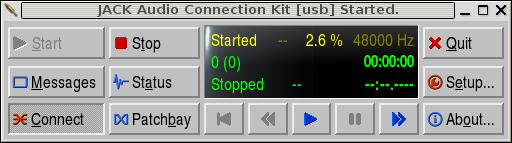
\includegraphics[width=10cm]{image200602/qjackctl-1.png}\\
managing jackd startup and connection
\end{frame}

\begin{frame}
 \frametitle{qjackctl managing MIDI}
 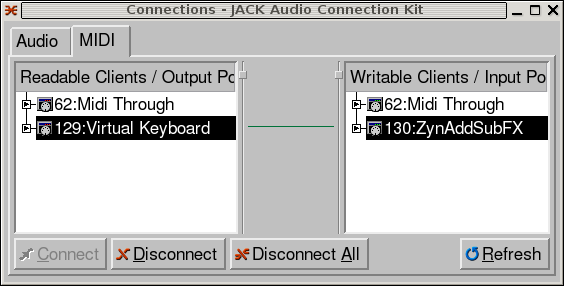
\includegraphics[width=10cm]{image200602/qjackctl-midi.png}\\
managing MIDI connections
\end{frame}

\begin{frame}
 \frametitle{qjackctl}
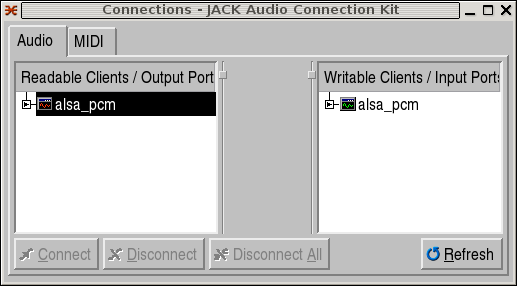
\includegraphics[width=10cm]{image200602/qjackctl-2.png}\\
 Jack connections
\end{frame}

\begin{frame}
 \frametitle{LADSPA effects}
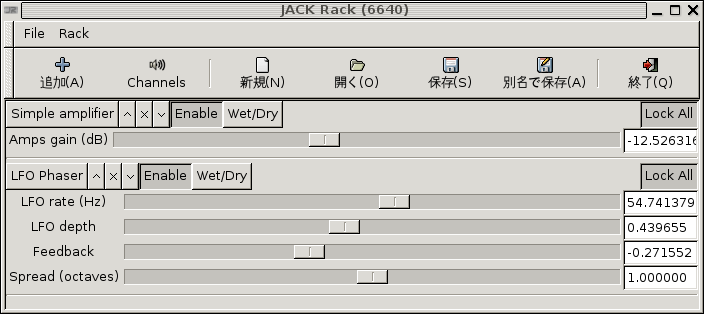
\includegraphics[width=10cm]{image200602/jack-rack.png}\\
input from jack audio, process with LADSPA effect, then output\\
There are several hundred effects available.
\end{frame}

\begin{frame}
 \frametitle{zynaddsubfx}
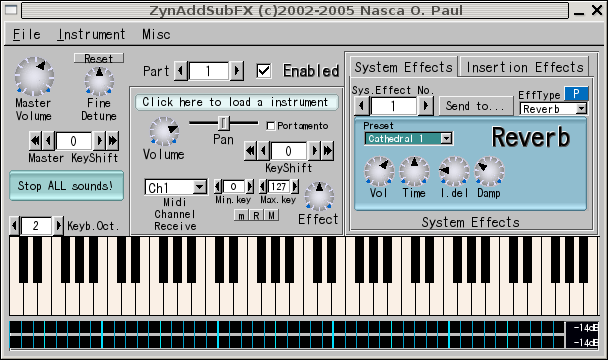
\includegraphics[width=10cm]{image200602/zynaddsubfx.png}
\end{frame}

\begin{frame}
 \frametitle{hydrogen}
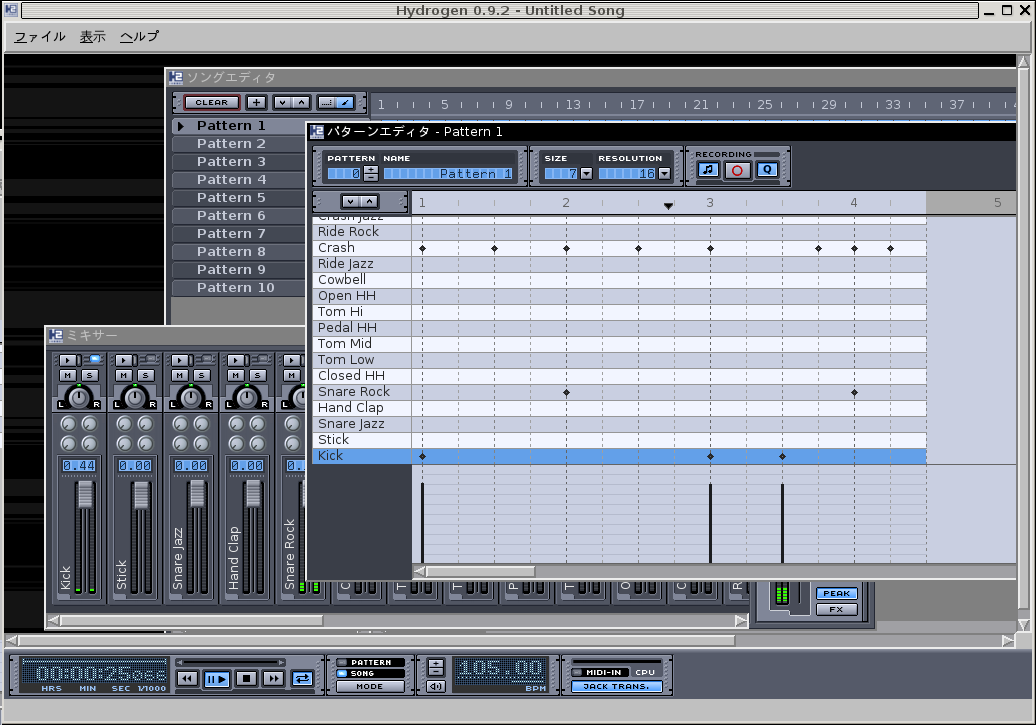
\includegraphics[width=10cm]{image200602/hydrogen.png}
\end{frame}

\begin{frame}
 \frametitle{rosegarden4}
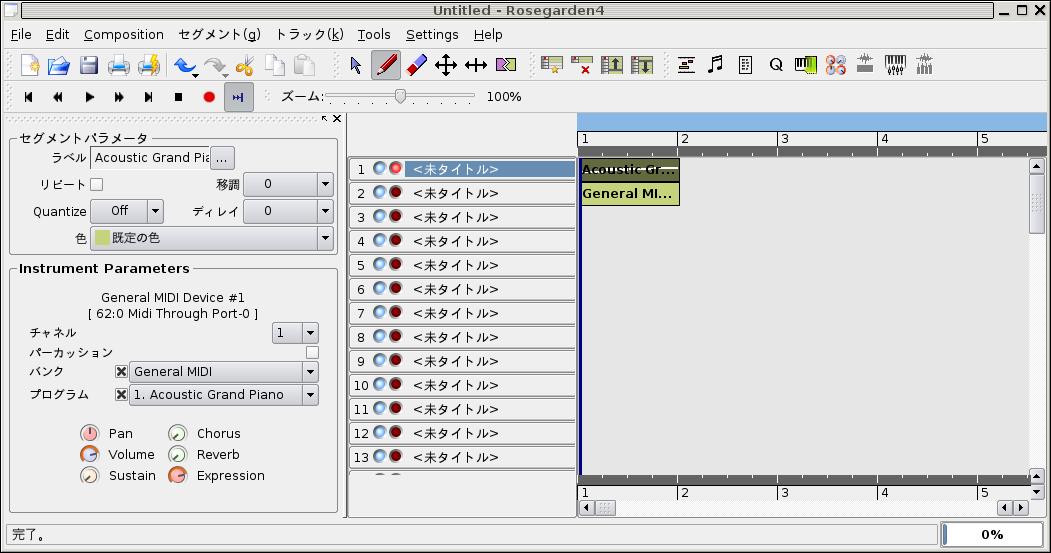
\includegraphics[width=10cm]{image200602/rosegarden4-1.png}
\end{frame}
\begin{frame}
 \frametitle{rosegarden4}
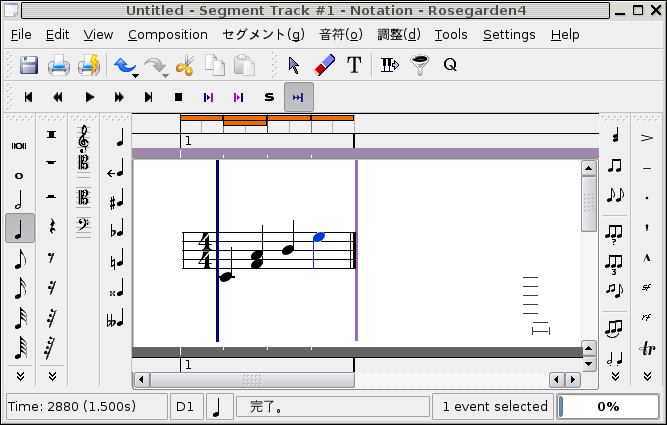
\includegraphics[width=10cm]{image200602/rosegarden4-2.png}
\end{frame}

\begin{frame}
 \frametitle{ardour}
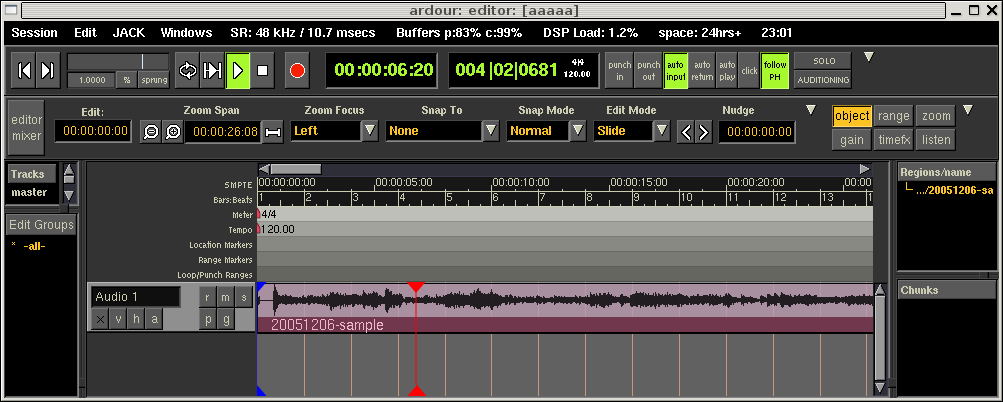
\includegraphics[width=10cm]{image200602/ardour2.png}
\end{frame}

\begin{frame}
 \frametitle{muse}
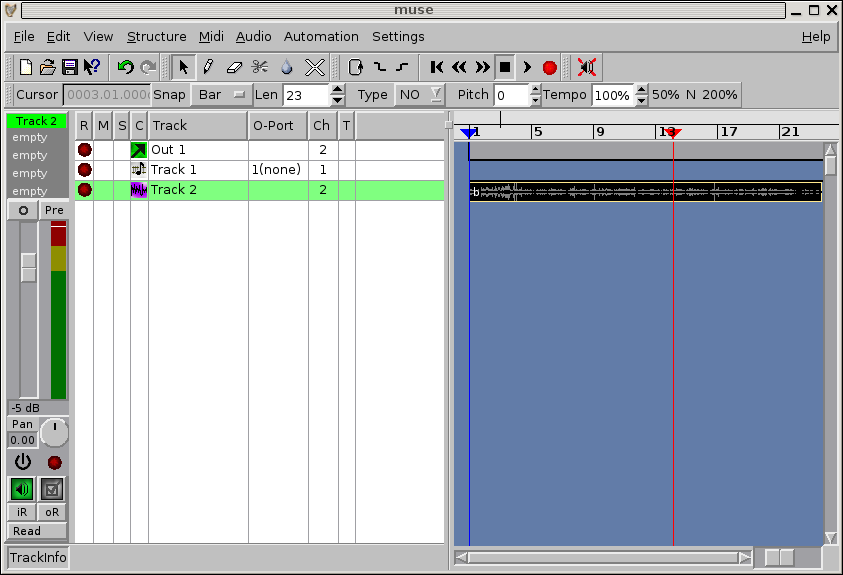
\includegraphics[width=10cm]{image200602/muse.png}
\end{frame}

 \subsection{Future?}
\begin{frame}
 \frametitle{Action Plans}
\begin{itemize}
 \item debian-multimedia-policy: Try to come up with a plan so that
       applications cooperate with each other. Unify default behaviour.
 \item demudi-to-debian merge: merge packages as necessary.
       Things such as kernel-patch-realtime-lowlatency required in
       Debian main.
 \item LASH: Automating the process of starting the applications and
       then connecting them. Currently, it's cumbersome.
 \item Quality assurance. 
       Want to start adding regression testsuites.
       Most of applications I don't know how to use; starting with researching
       the usage scenarios.
\end{itemize}

\end{frame}

\end{document}
